\clearpage
\appendix
% =================================================================
\section{Anexo: evidencias adicionales}
% =================================================================

\begin{figure}[H]
\centering
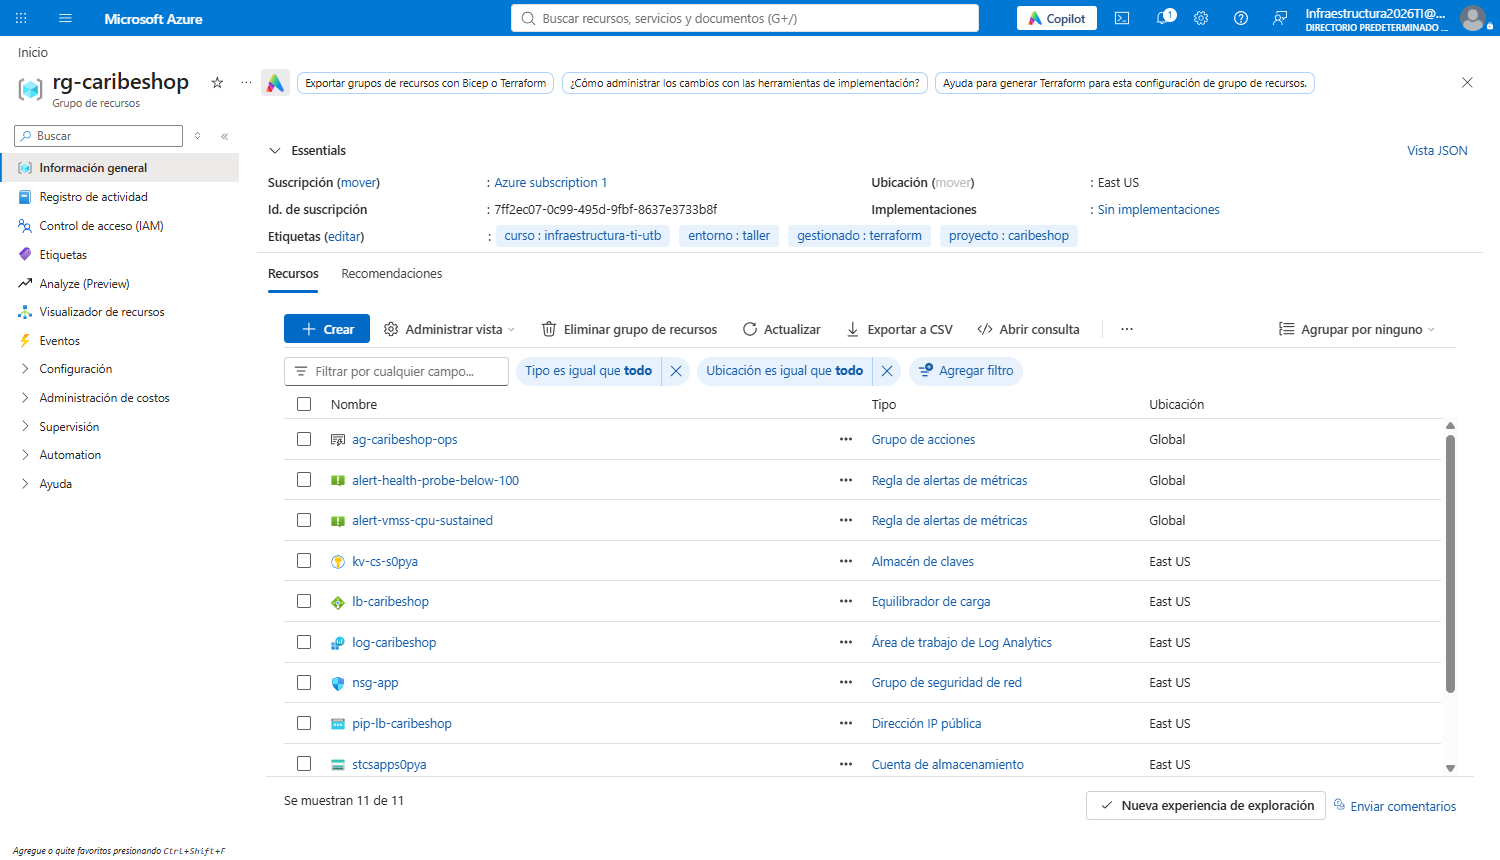
\includegraphics[width=0.9\textwidth]{figuras/01_rg_recursos.png}
\caption{Grupo de recursos \texttt{rg-caribeshop} con los recursos creados por Terraform.}
\end{figure}

\begin{figure}[H]
\centering
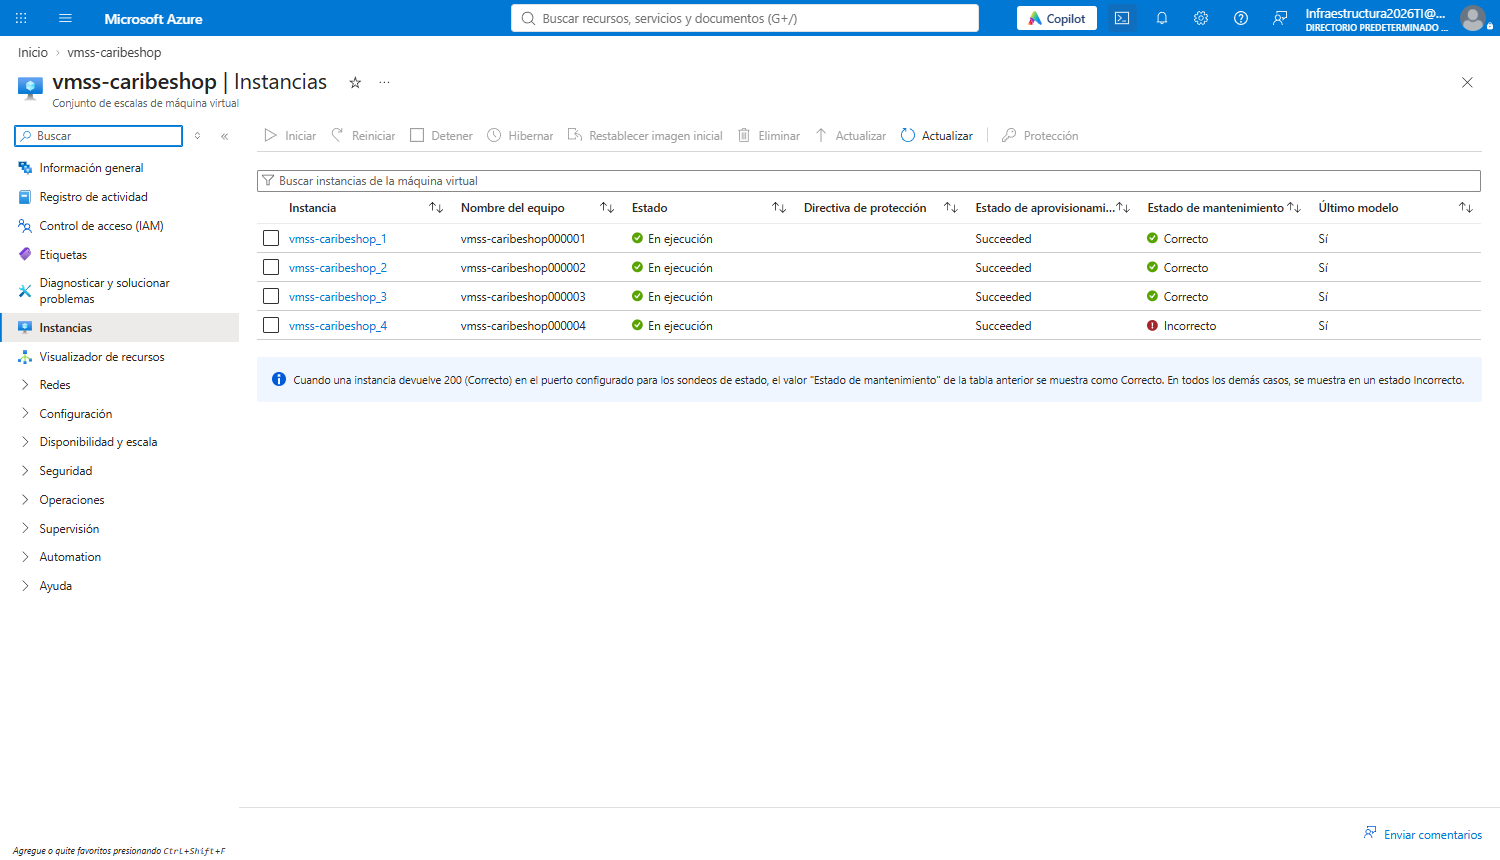
\includegraphics[width=0.9\textwidth]{figuras/13_vmss_instances.png}
\caption{E1/E3: VMSS con 4 instancias durante el pico de la prueba escalonada.}
\label{fig:vmss4}
\end{figure}

\begin{figure}[H]
\centering
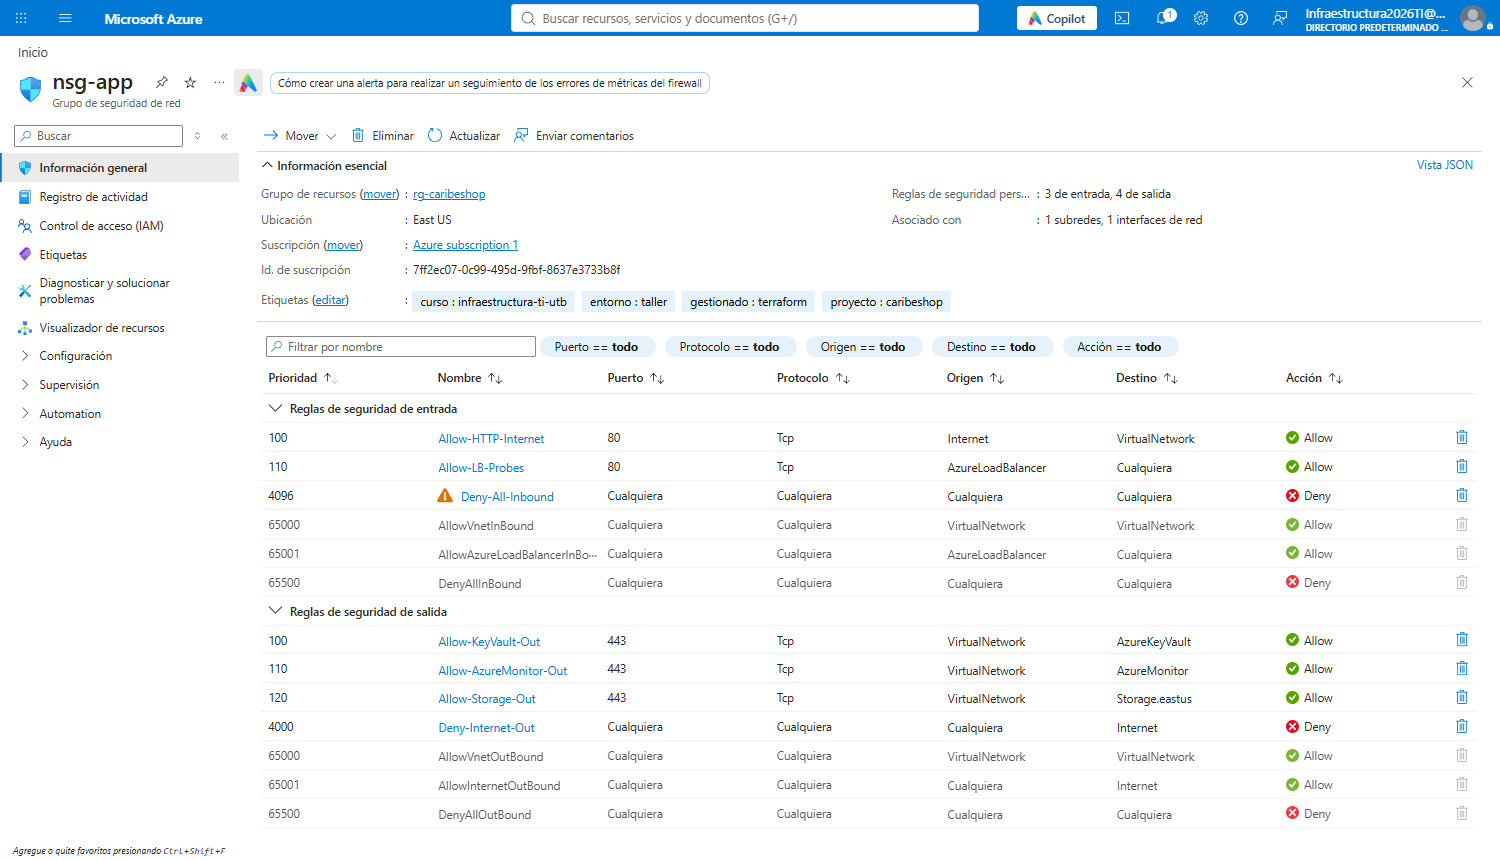
\includegraphics[width=0.9\textwidth]{figuras/04_nsg_reglas.png}
\caption{S2: reglas del NSG \texttt{nsg-app} (entrada solo 80; salida solo etiquetas de servicio).}
\label{fig:nsg}
\end{figure}

\begin{figure}[H]
\centering
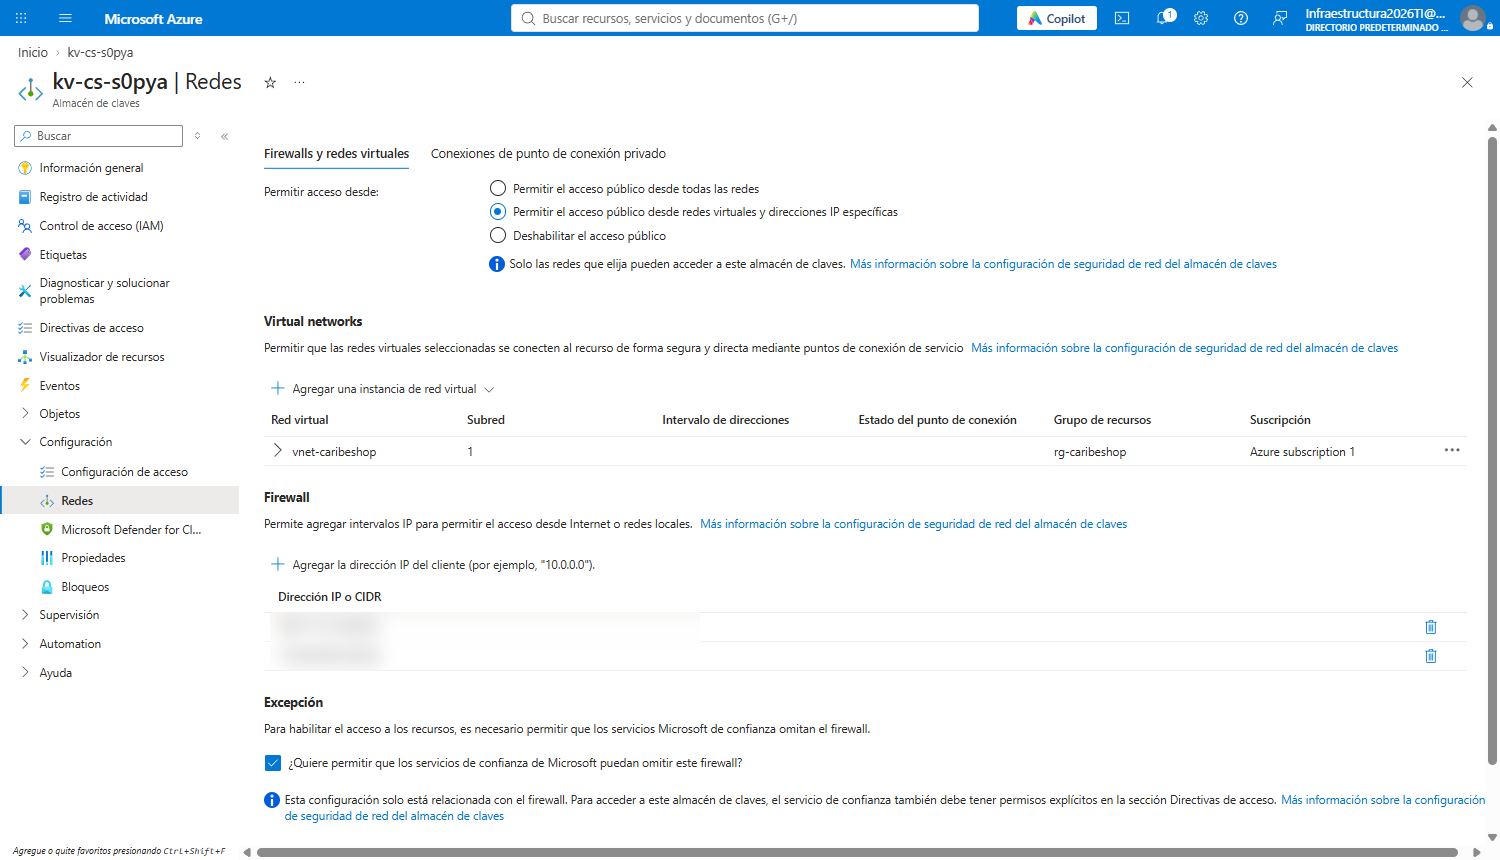
\includegraphics[width=0.9\textwidth]{figuras/05_kv_firewall.png}
\caption{S3: firewall del Key Vault (subred \texttt{snet-app} + rangos del operador).}
\label{fig:kvfw}
\end{figure}

\begin{figure}[H]
\centering
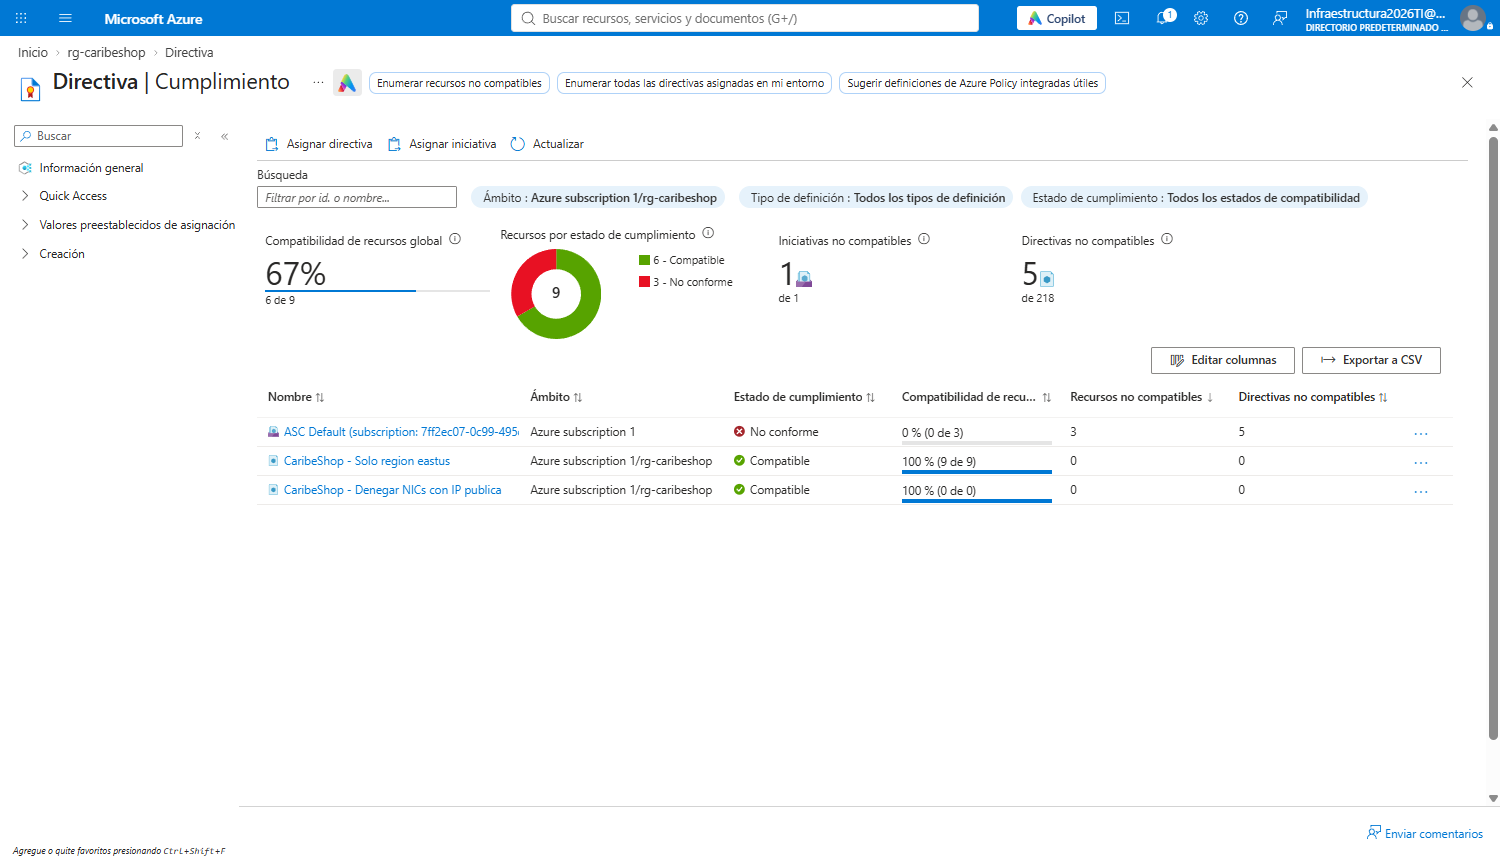
\includegraphics[width=0.9\textwidth]{figuras/07_politicas.png}
\caption{S5: asignaciones de Azure Policy en el grupo de recursos (cumplimiento).}
\end{figure}

\begin{figure}[H]
\centering
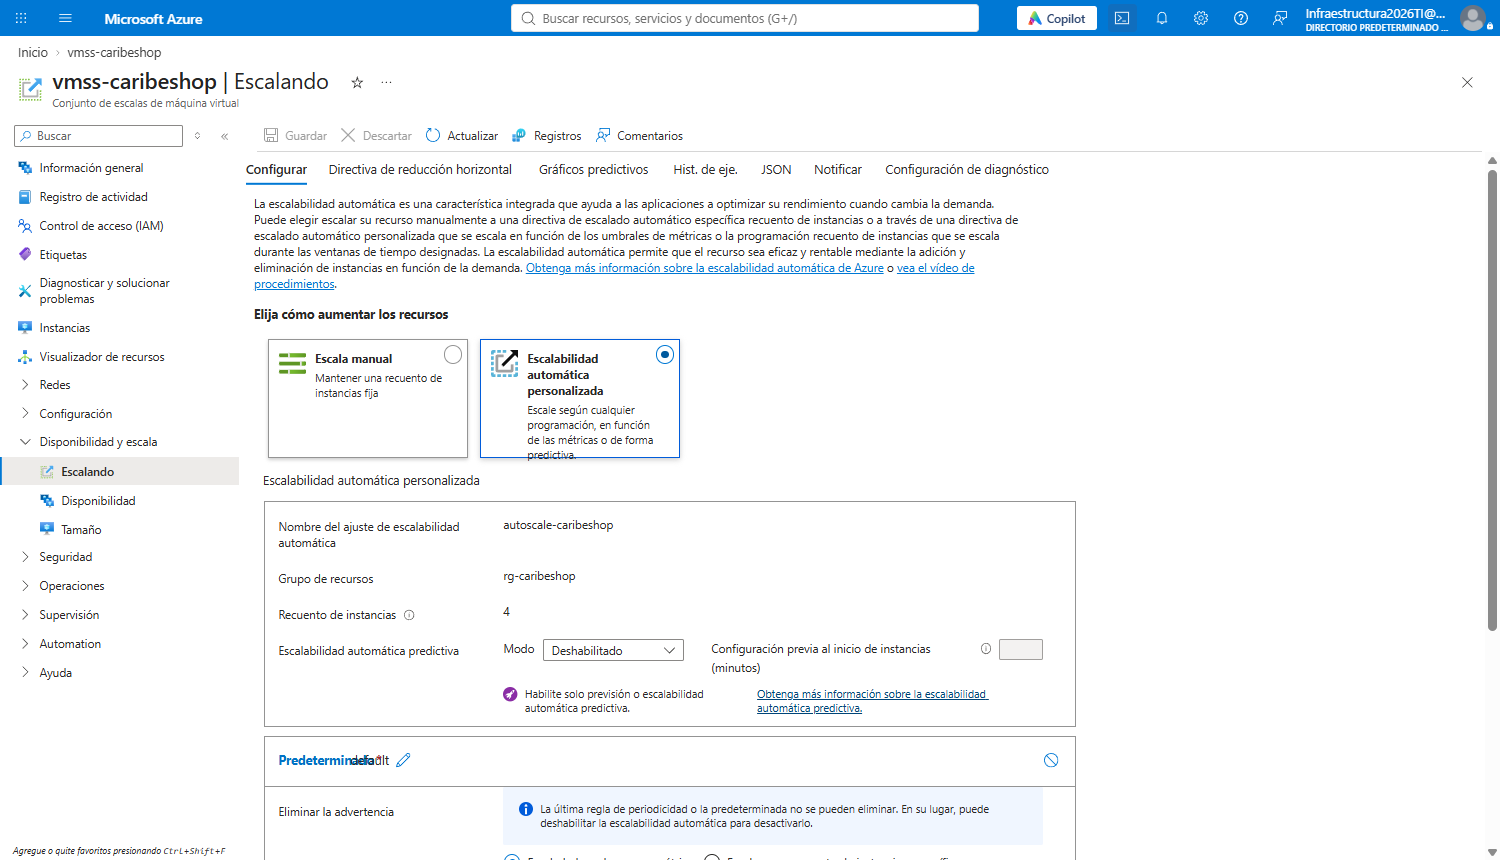
\includegraphics[width=0.9\textwidth]{figuras/08_autoscale.png}
\caption{E3: autoscale personalizado del VMSS (recuento de 4 instancias durante el pico).}
\end{figure}

\begin{figure}[H]
\centering
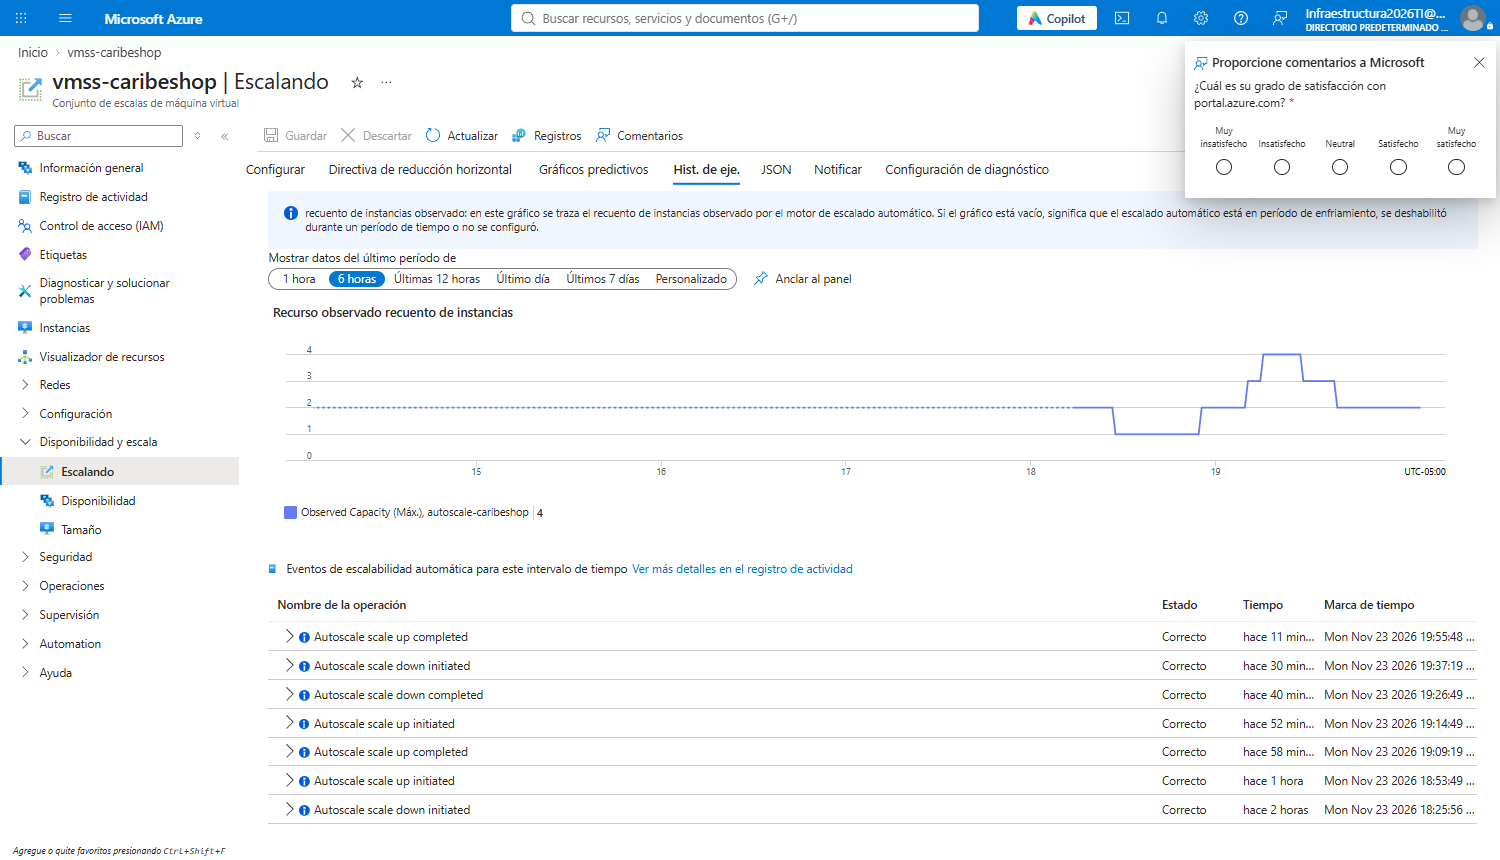
\includegraphics[width=0.9\textwidth]{figuras/16_e3_historial_autoscale.png}
\caption{E3: historial de ejecución del autoscale en el portal (2$\rightarrow$1 en P1.1; 2$\rightarrow$3$\rightarrow$4$\rightarrow$3$\rightarrow$2 en P1.2; 1$\rightarrow$2 en P2.2).}
\end{figure}

\begin{figure}[H]
\centering
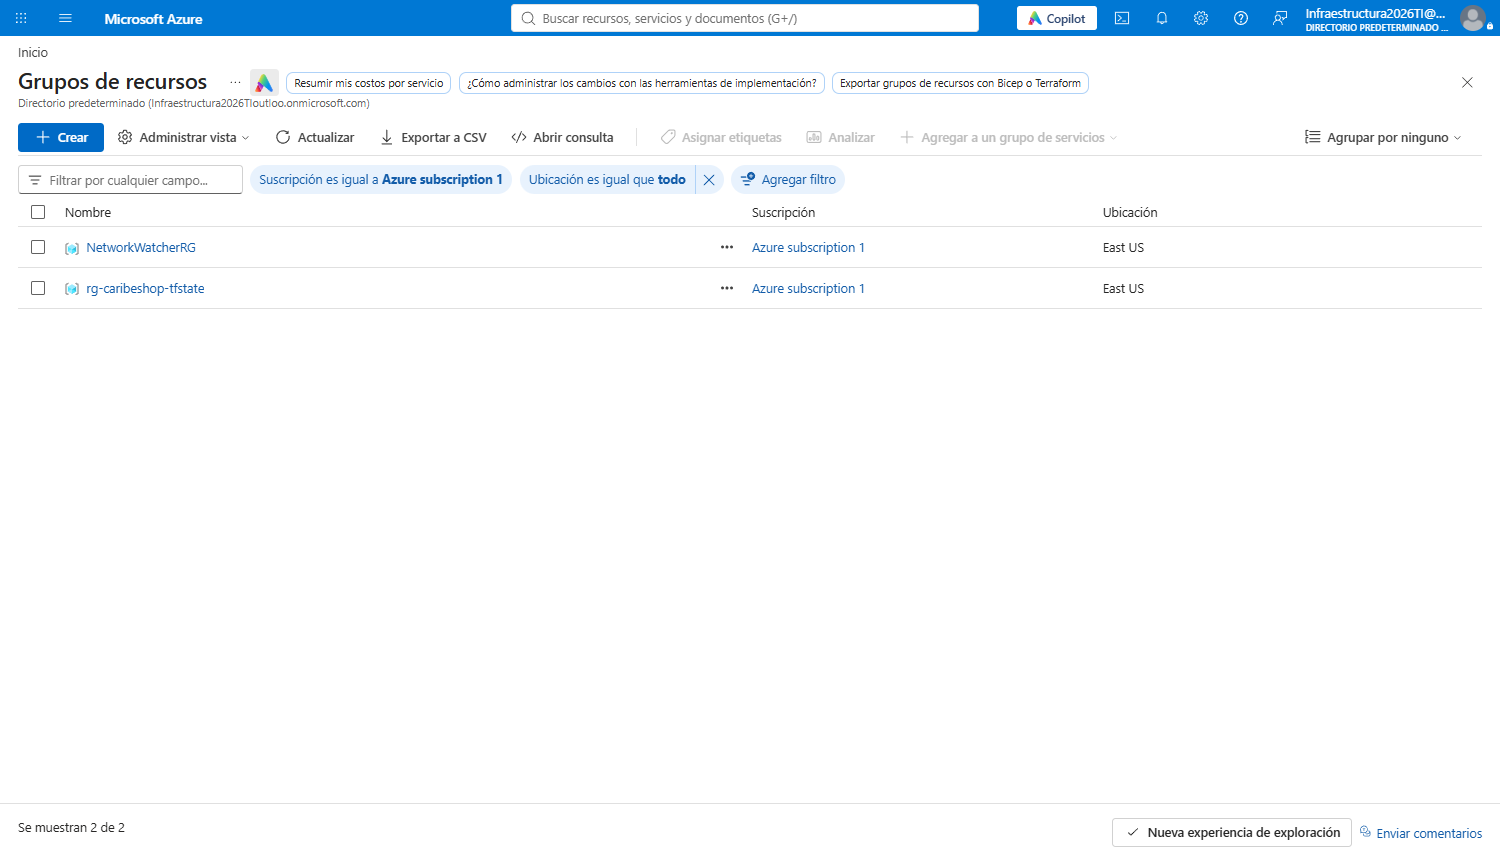
\includegraphics[width=0.9\textwidth]{figuras/21_destroy_verificado.png}
\caption{Verificación tras \texttt{terraform destroy} (33 recursos eliminados): solo queda el grupo del estado remoto; \texttt{NetworkWatcherRG} lo crea Azure automáticamente y está vacío.}
\end{figure}

\begin{figure}[H]
\centering
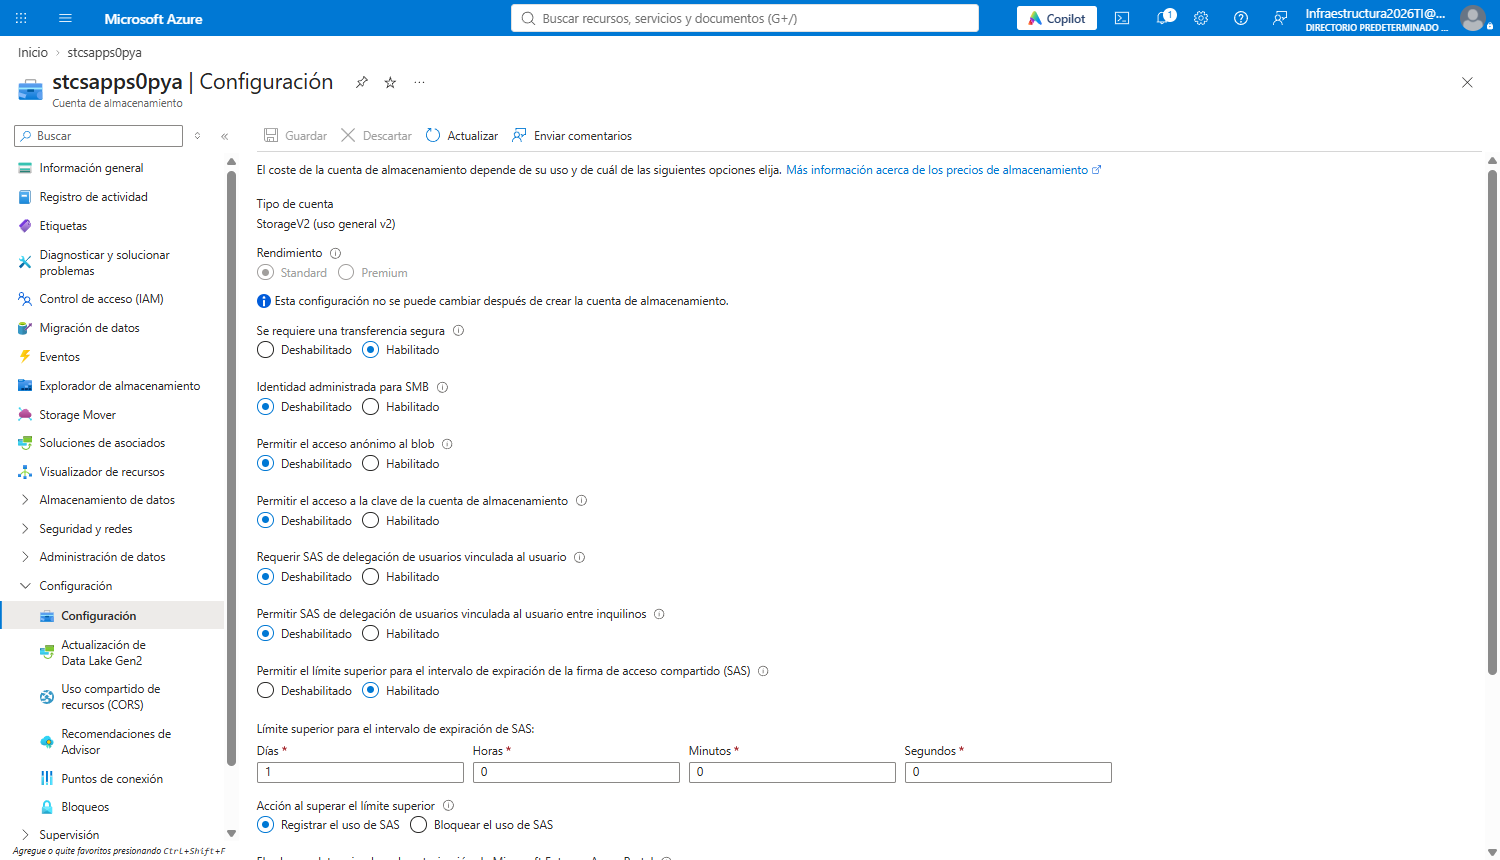
\includegraphics[width=0.9\textwidth]{figuras/11_storage_sin_llaves.png}
\caption{Storage de la app: acceso con llave compartida deshabilitado.}
\end{figure}

\begin{lstlisting}[caption={S2/S4: salidas de la CLI (extracto de \texttt{evidencias/cli/}).},language={}]
## az vmss nic list (instancias sin IP publica)
Nic      PrivateIp      PublicIp
nic-app  10.20.1.4      (ninguna)
nic-app  10.20.1.5      (ninguna)
## IPs publicas en el RG: solo pip-lb-caribeshop (Standard, zonas 1,2,3)

## az role assignment list --assignee 95df5c1c-3391-42db-be9e-5a322a5acad3 --all
Role                    Scope
Key Vault Secrets User  .../vaults/kv-cs-s0pya/secrets/db-password
\end{lstlisting}
